
%(BEGIN_QUESTION)
% Copyright 2013, Tony R. Kuphaldt, released under the Creative Commons Attribution License (v 1.0)
% This means you may do almost anything with this work of mine, so long as you give me proper credit

This Allen-Bradley PLC program takes inputs from multiple pushbutton switches to control the status of output bit {\tt O:0/2}:

$$\includegraphics[width=15.5cm]{i03357x01.eps}$$

Re-write this PLC program, using {\it retentive coil} instructions (i.e. ``Latch'' and ``Unlatch'' coils) instead of the single output coil in the original program.  Write your program such that the exact same physical pushbutton switches will work the same as with the old program -- in other words, so nothing needs to be replaced or re-wired to accommodate the differences in your new program:

$$\includegraphics[width=15.5cm]{i03357x02.eps}$$

\underbar{file i03357}
%(END_QUESTION)





%(BEGIN_ANSWER)

Full credit only for a solution that is complete with all correct addresses and instruction types.  If any address labels are missing, deduct half credit:

$$\includegraphics[width=15.5cm]{i03357x03.eps}$$

%(END_ANSWER)





%(BEGIN_NOTES)

{\bf This question is intended for exams only and not worksheets!}.

%(END_NOTES)


